\section{Realização da Busca e Seleção dos Artigos}

A execução da \textit{string} foi realizada em 23 de junho de 2024 utilizando a base de dados Scopus \cite{elsevier2022}. Considerando que, a literatura publicada até o ano de 2022 já havia sido mapeada no estudo de controle \cite{erthal_characterization_2023}, filtrou-se a pesquisa para após o referido ano, o que resultou em 283 estudos. Dos trabalhos deste primeiro grupo, foram lidos título e resumo, realizando uma filtragem seguindo o protocolo de pesquisa formalizado durante o planejamento. Este processo resultou na seleção de três estudos secundários (dentre eles o artigo de controle), apresentados na Tabela \ref{tab:resultados-busca}.

\begin{table}[h!]
    \caption{Estudos Selecionados dos Resultados da Execução da Busca}

    \begin{tabular}{|p{.5cm}|p{6cm}|p{6cm}|p{1.75cm}|}
        \hline
        Nº & Título & Fonte de Publicação & Referência \\ \hline
        1 & \textit{Characterization of Continuous Experimentation in Software Engineering: Expressions, models, and strategies} & \textit{Science of Computer Programming} & \cite{erthal_characterization_2023} \\ \hline
        2 & \textit{A/B testing: A Systematic Literature Review} & \textit{Journal of Systems and Software} & \cite{quin_b_2024} \\ \hline
        3 & \textit{Statistical Challenges in Online Controlled Experiments: A Review of A/B Testing Methodology} & \textit{The American Statisticia}n & \cite{larsen_statistical_2024} \\ \hline
    \end{tabular}
    
    \begin{center}
        \text{Fonte: Autor}
    \end{center}

    \label{tab:resultados-busca}
\end{table}

Tendo sido publicados em revistas científicas, os trabalhos se mostraram fontes de qualidade para se compreender o estado da arte e encontrar estudos primários na área da experimentação.

O primeiro, \citeonline{erthal_characterization_2023}, traz expressões, modelos e estratégias utilizadas pelos praticantes do desenvolvimento orientado a dados, propondo inclusive um processo, o chamado \textit{Combined Process for Continuous Experimentation}, que consolida as principais atividades a serem seguidas por aqueles que buscam implementar um processo de experimentação contínua.

O segundo, \citeonline{quin_automating_2024}, aborda o  \textit{design} e a execução de testes A/B e também o papel dos \textit{stakeholders} neste processo, algo importante no contexto deste trabalho. 

Já o terceiro, \citeonline{larsen_statistical_2024}, diferente dos dois anteriores, não utiliza um protocolo sistemático de busca na literatura, focando apenas em discutir atuais desafios estatísticos enfrentados pelos praticantes, trazendo exemplos e adentrando no domínio da literatura estatística.

Com o intuito de realizar o processo de \textit{snowballing}, durante a leitura dos artigos selecionados foram levantadas todas as referências citadas em tópicos relacionados as questões de pesquisa desta monografia. Após agrupar o material e eliminar as duplicações, foram separados 75 estudos primários. Destes, foi realizada a leitura parcial (título e resumo e, se necessário, introdução e conclusão) a fim de levantar apenas aqueles com informações pertinentes a alguma das questões de pesquisa. Esta atividade resultou na escolha de 20 artigos.

Após esta seleção, seguindo o protocolo da revisão estruturada, avançou-se para a etapa de Avaliação da Qualidade do material, onde foi verificada a fonte de publicação de cada trabalho com o intuito de levantar aqueles que foram publicados em alguma revista científica e os priorizar no processo de leitura completa do material. O grupo final de artigos consolidado é apresentado na Tabela \ref{tab:conjunto-final}. Este processo é visualmente apresentado na Figura \ref{fig:selecao}, demonstrando quantos artigos foram lidos integralmente e quantos foram selecionados em cada fase.

Desta forma, todo o processo de busca resultou na leitura de 29 artigos, sendo 7 do conjunto inicial (Tabela \ref{tab:conjunto-inicial}), 3 da execução da \textit{string} de busca (Tabela \ref{tab:resultados-busca}, aqui o artigo de controle não conta, já que fez parte do conjunto inicial) e 20 por \textit{snowballing}, onde 4 vieram da revisão da literatura de \citeonline{quin_b_2024} \cite{yu_new_2020} \cite{chen_automatic_2018} \cite{fabijan_benefits_2017} \cite{le_goues_towards_2014} e 16 do trabalho de \citeonline{erthal_characterization_2023} \cite{kuhrmann_activity_2018} \cite{bures_infrastructure_2021} \cite{kevic_characterizing_2017} \cite{liu_enterprise-level_2019} \cite{olsson_opinions_2014} \cite{fernandes_hitting_2015} \cite{melegati_hypotheses_2019} \cite{kohavi_online_2013} \cite{crook_seven_2009} \cite{issa_mattos_hurrier_2023} \cite{fabijan_online_2020} \cite{fagerholm_right_2017} \cite{fabijan_three_2019} \cite{olsson_towards_2015} \cite{sauvola_towards_2015} \cite{melegati_understanding_2021}
.

A maioria dos estudos selecionados foi extraída do artigo de \citeonline{erthal_characterization_2023}, uma vez que, por ter sido publicado anteriormente e por se propor a caracterizar a literatura existente, a maior parte do material selecionado, mesmo que citada em algum dos outros dois artigos, já havia sido mapeado pelos autores.

Não houve inclusão de artigos provenientes das citações de \citeonline{larsen_statistical_2024}, pois, por não se tratar de um mapeamento da literatura, o estudo não apresenta os artigos primários de forma sistemática (como em tabelas, por exemplo). Por essa razão, optou-se por não utilizar as citações do referido estudo, já que seria necessário revisar todas as fontes mencionadas, uma quantidade inviável dada a limitação de tempo no contexto deste trabalho.

\todo[inline, color=pink]{REESCREVER o parágrafo anterior. Não foi por isso que ele não houve inclusão de outros estudos a partir dele, mas sim como gestão do tempo. Outra questão é que o fato de não utilizar protocolo da revisão sistemática não é justificativa para não escolha. O paper foi puplicado em revista. Além disso, ele é citado em relação a resposta dos principais problemas e desafios.}

\begin{figure}
    \centering
    \caption{Representação Visual da Seleção dos Artigos}
    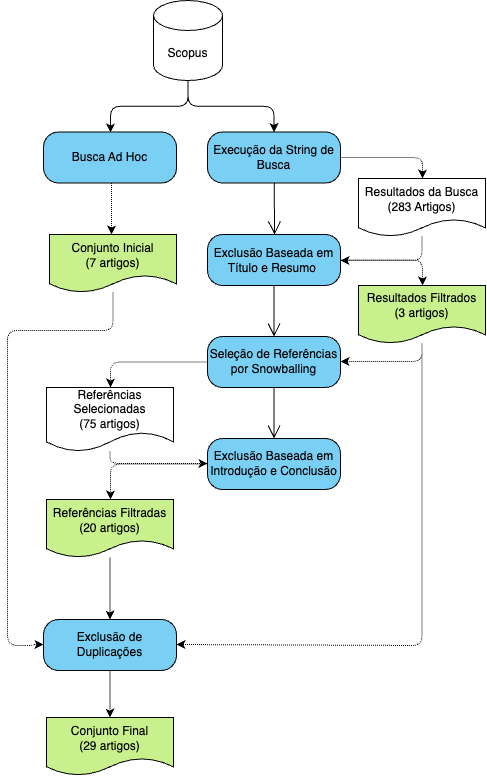
\includegraphics[width=0.7\linewidth]{figuras/selecao.png}
    \begin{center}
        \text{Fonte: Autor}
    \end{center}
    \label{fig:selecao}
\end{figure}

\begin{table}[]
    \caption{Conjunto Final de Artigos}
    
    \begin{tabular}{|p{.5cm}|p{6cm}|p{4cm}|p{4cm}|}
        \hline
        Nº & Título & Publicado em revista? & Referência \\ \hline
        1 & \textit{A New Framework for Online Testing of Heterogeneous Treatment Effect} & Não & \citeonline{yu_new_2020} \\ \hline
        2 & \textit{A/B testing: A Systematic Literature Review} & Sim & \citeonline{quin_b_2024} \\ \hline
        3 & \textit{An Activity and Metric Model for Online Controlled Experiments} & Não & \citeonline{kuhrmann_activity_2018} \\ \hline
        4 & \textit{An Infrastructure for Platform-Independent Experimentation of Software Changes} & Não & \citeonline{bures_infrastructure_2021} \\ \hline
        5 & \textit{Automatic Detection and Diagnosis of Invalid Online Experiments} & Não & \citeonline{chen_automatic_2018} \\ \hline
        6 & \textit{Characterization of Continuous Experimentation in Software Engineering: Expressions, Models and Strategies} & Sim & \citeonline{erthal_characterization_2023} \\ \hline
        7 & \textit{Characterizing Experimentation in Continuous Deployment: A Case Study on Bing} & Sim & \citeonline{kevic_characterizing_2017} \\ \hline
        8 & \textit{Enterprise-Level Controlled Experiments at Scale: Challenges and Solutions} & Não & \citeonline{liu_enterprise-level_2019} \\ \hline
        9 & \textit{From Opinions to Data-Driven Software R\&D: A Multi-case Study on How to Close the 'Open Loop' Problem} & Não & \citeonline{olsson_opinions_2014} \\ \hline
        10 & \textit{Hitting the target: Practices and Steps for moving toward innovation experiment systems} & Não & \citeonline{fernandes_hitting_2015} \\ \hline
        11 & \textit{Hypotheses Engineering: First Essential Steps of Experiment-Driven Software Development} & Não & \citeonline{melegati_hypotheses_2019} \\ \hline
        12 & \textit{Online Controlled Experiments at Large Scale} & Não & \citeonline{kohavi_online_2013} \\ \hline
        \multicolumn{4}{|c|}{Continua na Tabela \ref{tab:conjunto-final-2}} \\ \hline
    \end{tabular}
    
    \begin{center}
        \text{Fonte: Autor}
    \end{center}

    \label{tab:conjunto-final}
\end{table}

\begin{table}[]
    \caption{Continuação do Conjunto Final de Artigos}
    
    \begin{tabular}{|p{.5cm}|p{6cm}|p{4cm}|p{4cm}|}
        \hline
        \multicolumn{4}{|c|}{Continuação da Tabela \ref{tab:conjunto-final}} \\ \hline
        Nº & Título & Publicado em revista? & Referência \\ \hline
        13 & \textit{Seven Pitfalls to Avoid When Running Controlled Experiments on the Web} & Não & \citeonline{crook_seven_2009} \\ \hline
        14 & \textit{Statistical Challenges in Online Controlled Experiments: A Review of A/B Testing Methodology} & Sim & \citeonline{larsen_statistical_2024} \\ \hline
        15 & \textit{The Benefits of Controlled Experimentation at Scale} & Não & \citeonline{fabijan_benefits_2017} \\ \hline
        16 & \textit{The HURRIER process for experimentation in business-to-business mission-critical systems} & Sim & \citeonline{issa_mattos_hurrier_2023} \\ \hline
        17 & \textit{The Online Controlled Experiment Lifecycle} & Sim & \citeonline{fabijan_online_2020} \\ \hline
        18 & \textit{The RIGHT Model for Continuous Experimentation} & Sim & \citeonline{fagerholm_right_2017} \\ \hline
        19 & \textit{Three Key Checklists and Remedies for Trustworthy Analysis of Online Controlled Experiments at Scale} & Não & \citeonline{fabijan_three_2019} \\ \hline
        20 & \textit{Towards Automated A/B Testing} & Não & \citeonline{le_goues_towards_2014} \\ \hline
        21 & \textit{Towards Continuous Customer Validation: A Conceptual Model for Combining Qualitative Customer Feedback with Quantitative Customer Observation} & Não & \citeonline{olsson_towards_2015} \\ \hline
        22 & \textit{Towards Customer-centric Software Development: A Multiple-case Study} & Não & \citeonline{sauvola_towards_2015} \\ \hline
        23 & \textit{Understanding Hypotheses Engineering in Software Startups through a Gray Literature Review} & Sim & \citeonline{melegati_understanding_2021} \\ \hline
    \end{tabular}
    
    \begin{center}
        \text{Fonte: Autor}
    \end{center}

    \label{tab:conjunto-final-2}
\end{table}


